
\section{Schedule}

A Gannt chart detailing the timelines for each task
  is shown in figure~\ref{fig:schedule}.
In this section we describe the different phases 
  in some detail.


We have already started the project by looking how
  easy it is to write vector add in Java such that
  it uses the same file format and timing constructs
  as Parboil.
Both vector addition and matrix multiplication have
  already been ported to Java to examine the feasability
  of the project.
We have also already contacted the Renderscript team
  to understand what reasources and services they can
  provide in terms of hardware.

For the first phase of the project, we plan on porting
  4 of the simplest 


For the second phase of the project, we plan on porting
  4 of the simplest 

For the first phase of the project, we 

\begin{figure}[t!]
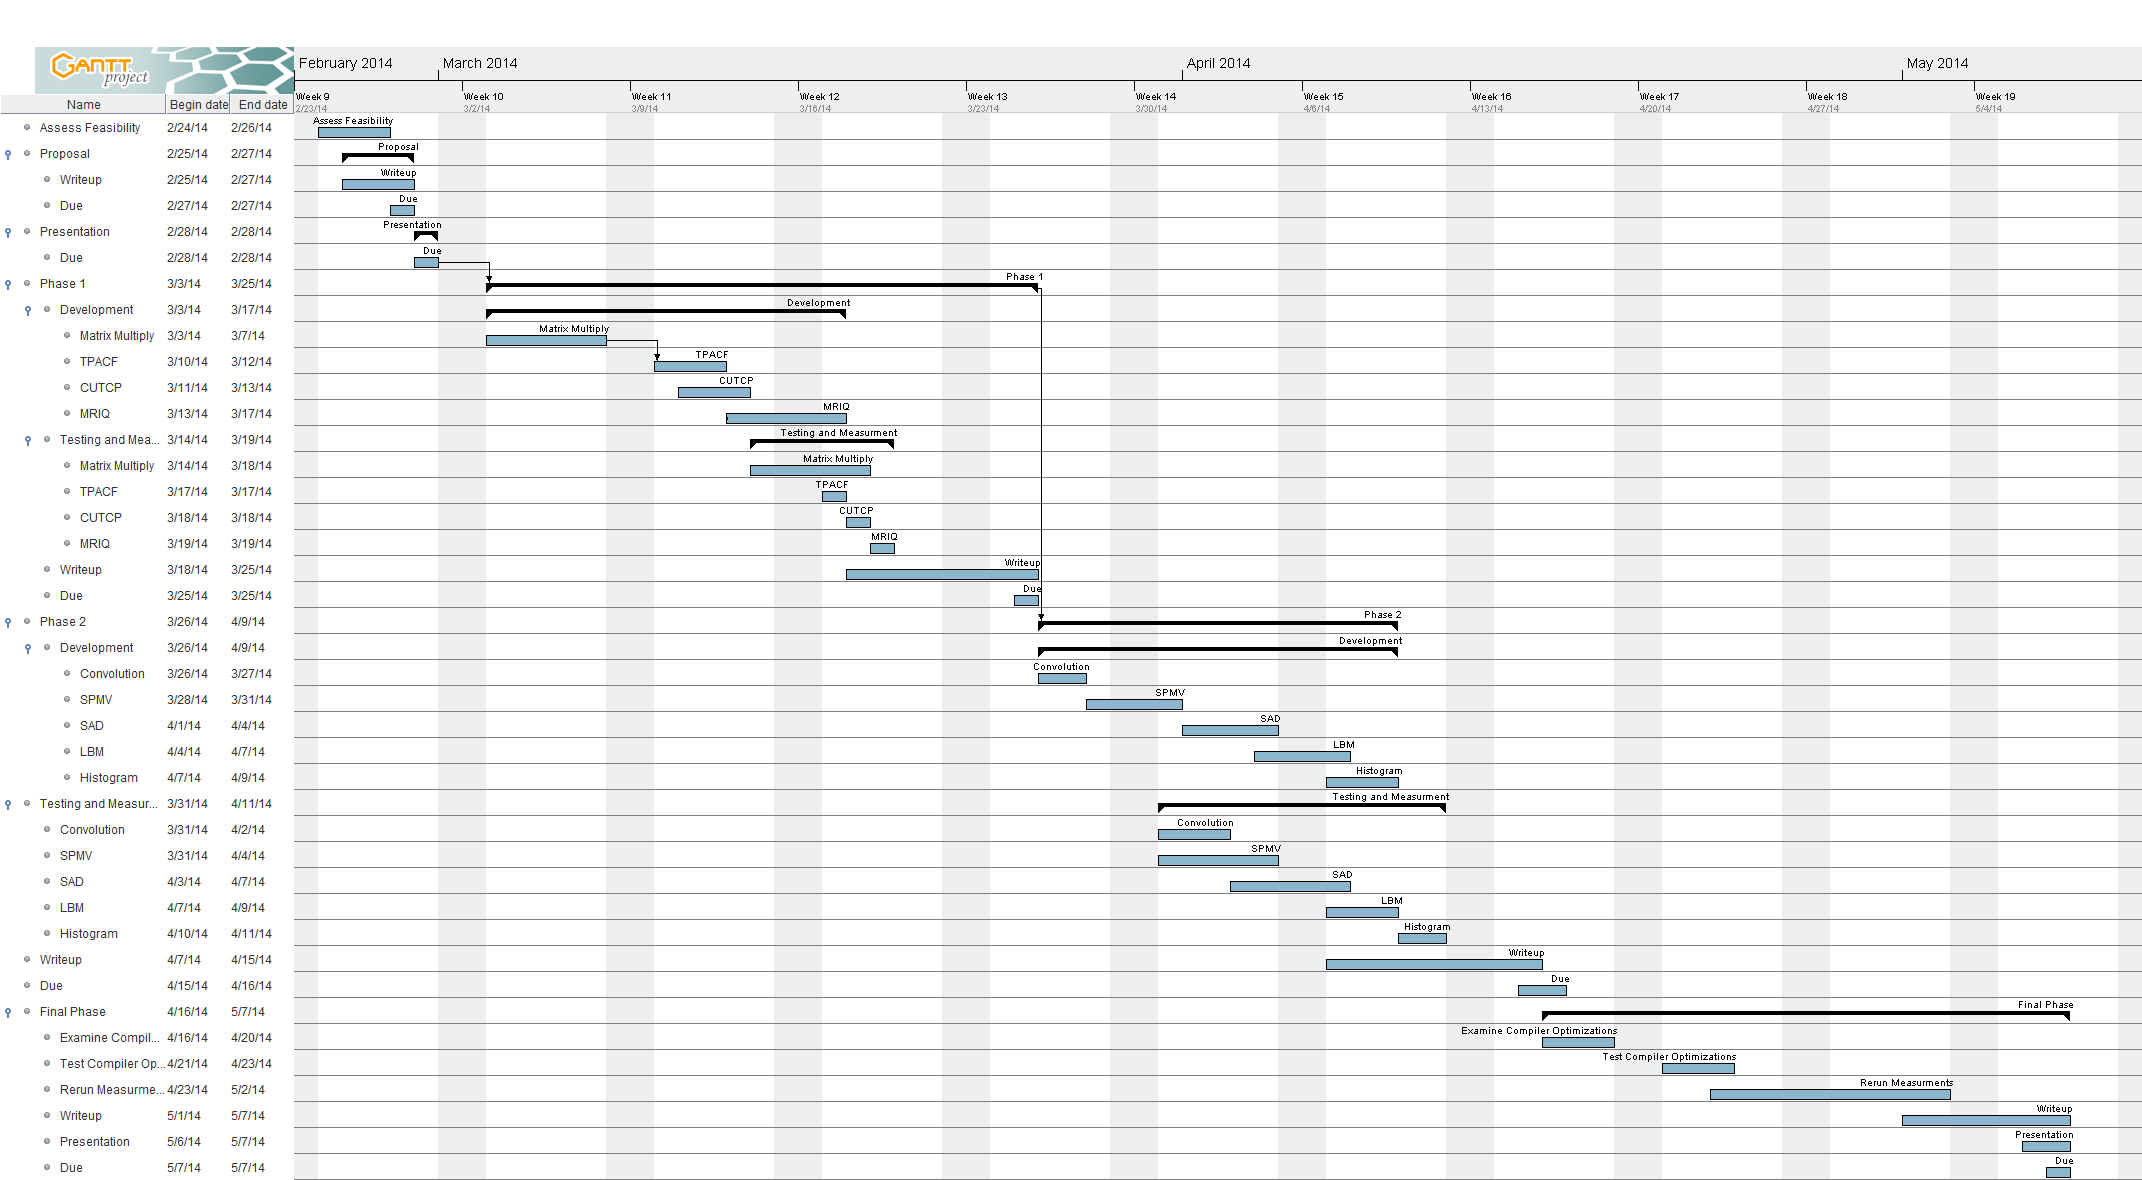
\includegraphics[scale=0.2, angle=90]{chart.png}
\caption{Projected project schedule.}
\label{fig:schedule}
\centering
\end{figure}